\chapter{Task execution}
In its most basic implementation, sensors and actuators can be directly tied to each other, removing the need for computation. Such robots are purely reactive, thereby missing the ability to ``think'' or plan. In order to achieve more complex behavior, memory and state are needed to switch between different controllers and algorithms.

This chapter introduces these basic principles as well as their implementation, starting with basic reactive controllers (Section \ref{sec:braitenberg}), then introduces more advanced concepts that let the robot make basic ``if'' \ldots ``then'' decisions using ``Finite State Machines'' (FSM) in Sections \ref{sec:fsm} and \ref{sec:stateflow}, and finally introduces advanced concepts such as ``behavior trees'' and semantic planning in Sections \ref{sec:behaviortrees} and \ref{sec:strips}.

\section{Reactive control}\label{sec:braitenberg}
A large variety of robotic behaviors can be accomplished by directly connecting sensor input to actuator output. These behaviors can even be accomplished without a computer, instead using analog electronics that provide appropriate conditioning. Simple autonomous robots using this concept have been demonstrated as early as 1953 \cite{walter1953living} and have become known as ``tortoises''. For example, by tying the output of a light sensor to a motor controller, the motor turns faster when the light is brighter. Using an inverse relationship, the motor will turn slower when the light is brighter. When used in a differential wheel configuration with two motors and two light sensors, such a robot either drives toward or away from the light. Formally, we can express the light following behavior, also known as \emph{phototaxis}\index{Phototaxis}, by the following relationship between 
the left and right wheel speeds, $\dot{\phi_l}$ and $\dot{\phi_r}$, and the measurements of the right and left light sensors, $\lambda_r$ and $\lambda_l$
\begin{eqnarray}\label{eq:simplereactive}
\dot{\phi_l}=a \lambda_r + b\\
\dot{\phi_r}=a \lambda_l + b
\end{eqnarray}
with $a$ a constant weight, and $b$ a bias term. We observe that the left wheel turns faster, the brighter the light shines on the right sensor. If the right light sensor receives more light than the left sensor, the right wheel will turn slower, resulting into a right turn, thereby exhibiting phototaxis behavior.

\begin{figure}
\centering
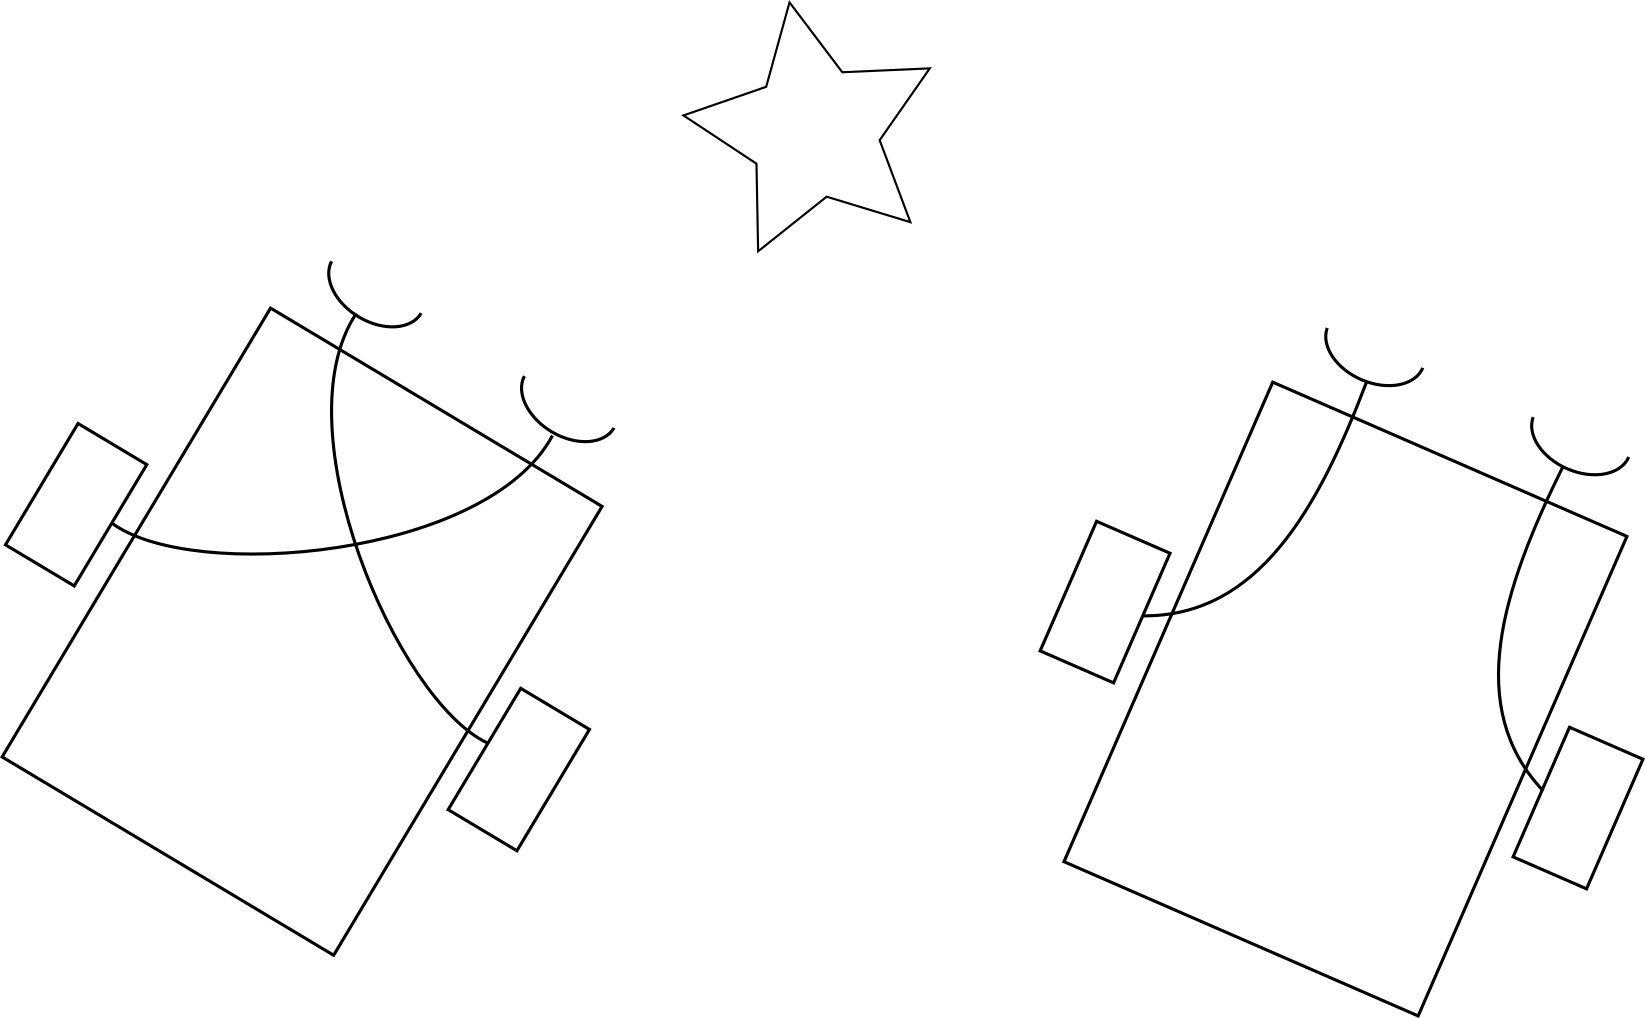
\includegraphics[width=0.7\columnwidth]{figs/braitenberg.png}
\caption{Two vehicles approaching a light source. The brighter the light, the more does each motor turn. The left vehicle will therefore approach the light by turning toward it, the right vehicle will avoid it by turning away from it.\label{fig:braitenberg}}
\end{figure}

A more complex behavior is obstacle avoidance. Assuming the output of an obstacle sensor to increase with the obstacle approaching (e.g., an infrared proximity sensor), we can use the same principle to compute the wheel speeds such that the obstacle is actively avoided. An example for a differential-wheel robot with eight infrared proximity sensors is given by
\begin{eqnarray}
\nonumber
\dot{\phi_l}&=&-6d_0-6d_1-19d_2-13d_3+94d_4+63d_5-50d_6-6d_7+b\\
\nonumber
\dot{\phi_r}&=&-6d_0+50d_1+63d_2+94d_3-22d_4-10d_5-6d_6-6d_7+b
\end{eqnarray}
%
% back, left {-0.06, -0.06}, 
% left {-0.06, 0.5}, 
% front, left {-0.19, 0.63}, 
% front, front, left{-0.13, 0.942}
% front, front, right {0.942, -0.22}, % left right motor
% front, right {0.63, -0.1}, 
% right {0.5, -0.06},  
% back, right {-0.06, -0.06},
%
with $d_0$ as the left rearward sensor and the other sensors being arranged clockwise such that $d_7$ is the right rearward sensing sensor, arranged as on the E-Puck differential wheel robot \cite{mondada2009puck}, see also Figure \ref{fig:epucksensors}.

\begin{figure}
\centering
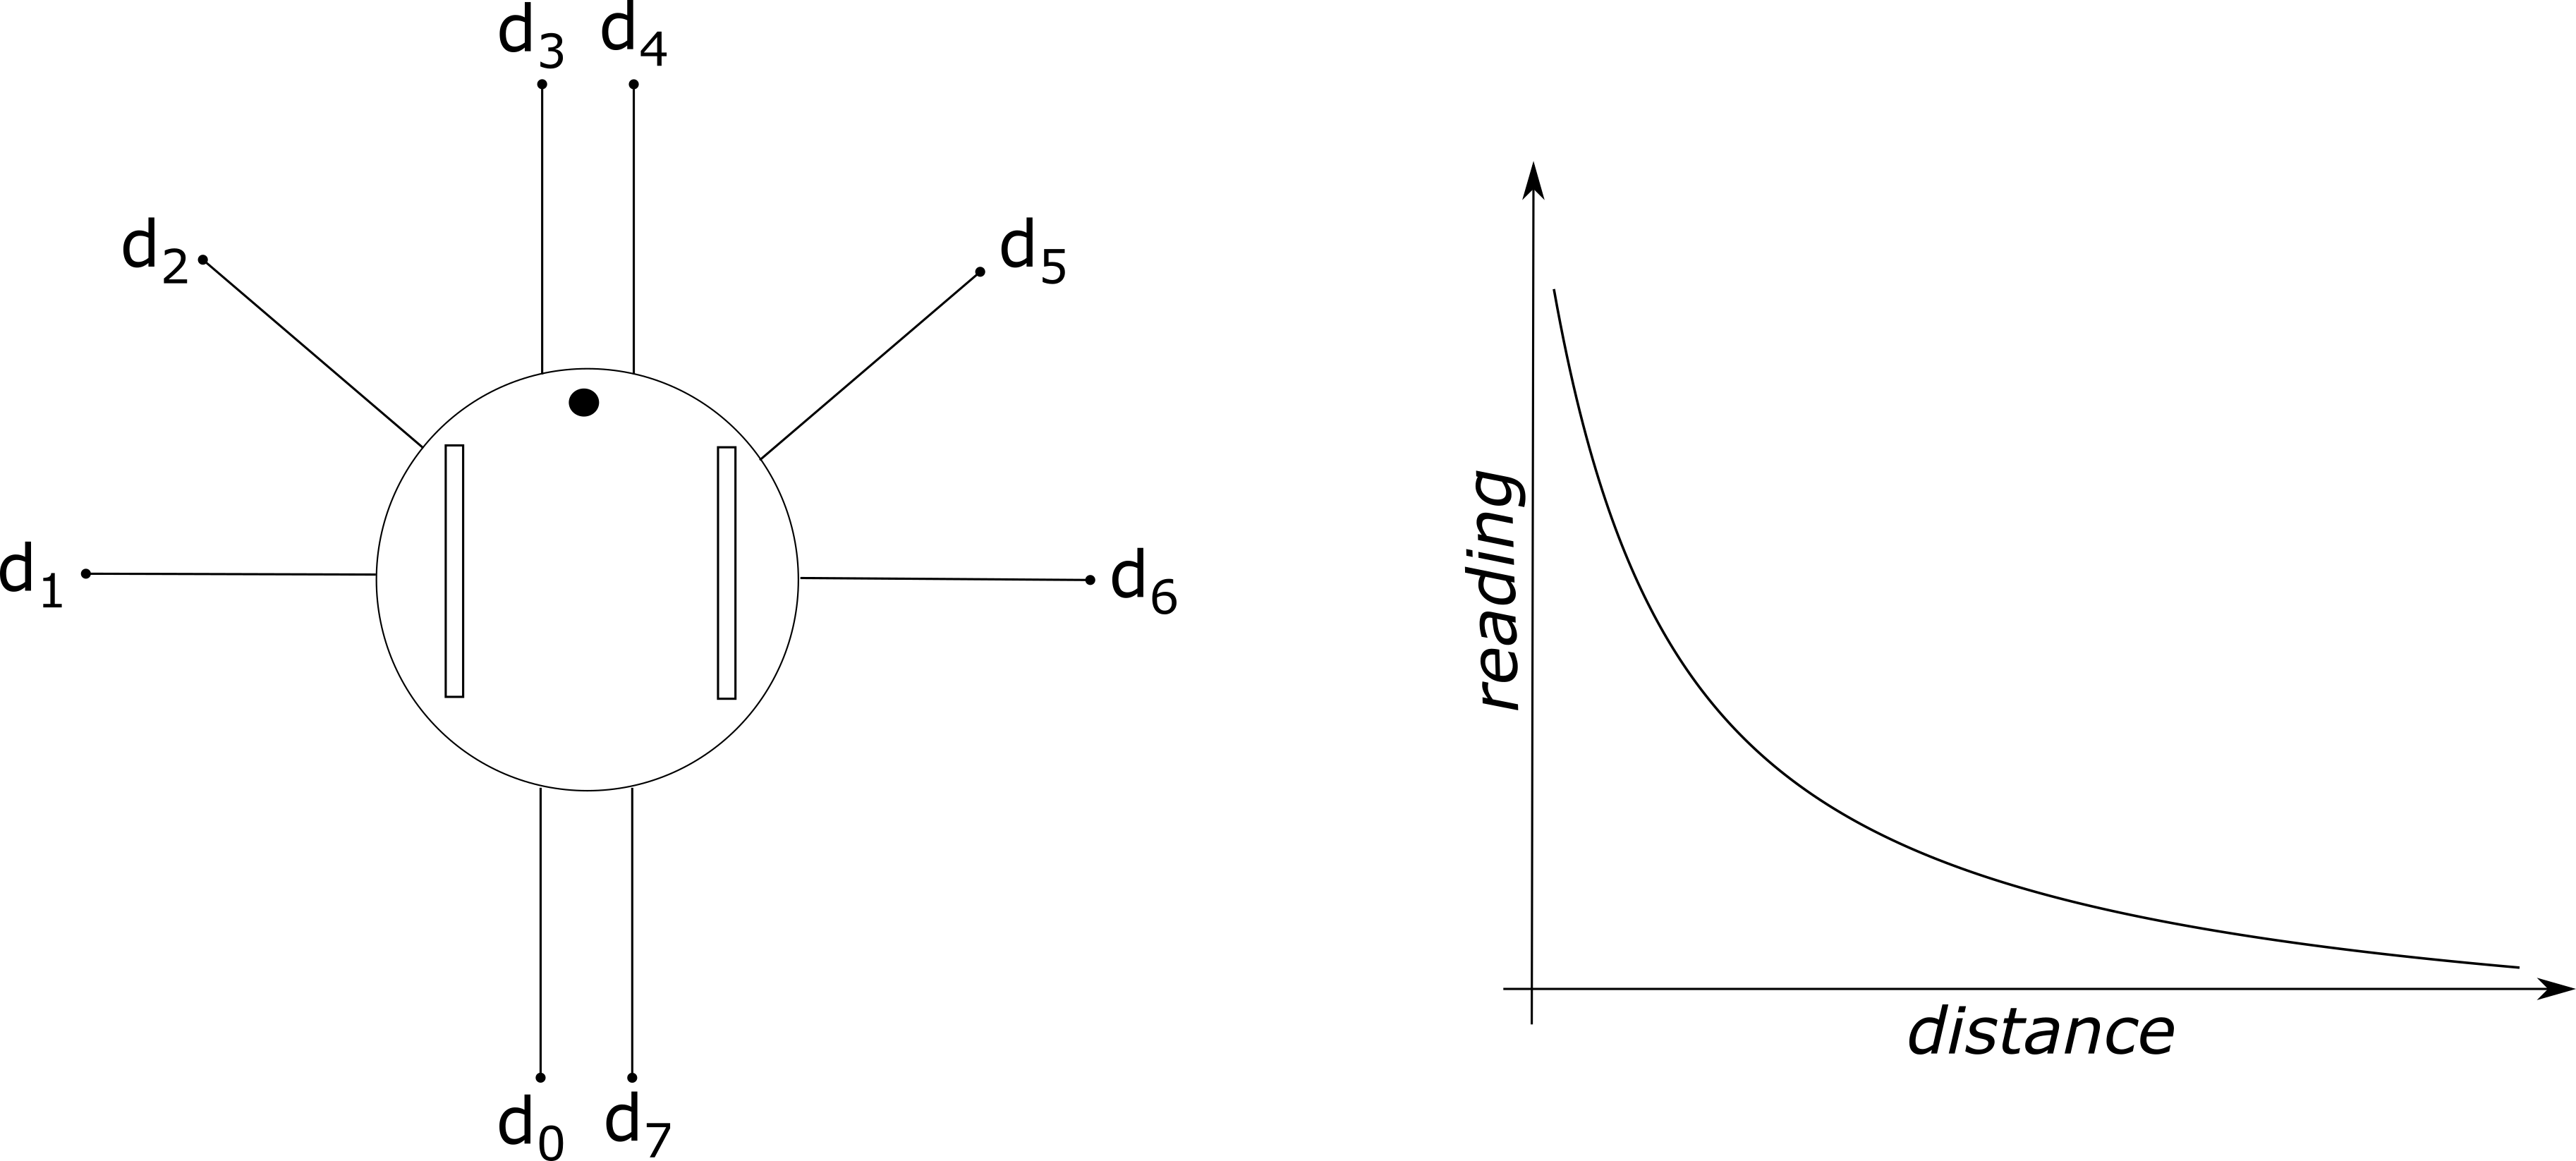
\includegraphics[width=0.9\columnwidth]{figs/ePuck.png}
\caption{\ref{fig:epucksensors}A schematic of a differential-wheel robot with eight infrared distance sensors (left) and typical sensor response as a function of distance (right).}
\end{figure}

Behaviors such as phototaxis and obstacle avoidance can also be combined by simply adding them and weighing each input accordingly. This idea has been popularized by the neuroscientist Valentino Braitenberg who augmented this system with additional ideas around learning (changing the weights based on events such as collisions), natural selection (building robots with random weights and selecting those that perform best), and analogies to the human brain \cite{braitenberg1986vehicles}. Controllers of these kind are therefore often called ``Braitenberg''.

Indeed, the controllers above bear strong resemblance to artificial neural networks such as described in Chapter \ref{chap:anns}, and ``optimal'' values to obtain a certain behavior can be obtained using evolutionary computation \cite{floreano1998evolutionary} or by training a neural network that yields appropriate input/output pairs. 

There are numerous variants of the control architecture including the \emph{subsumption architecture} \cite{brooks1990elephants} and \emph{motor schemas} \cite{arkin1989motor} that propose variations of switching different components of a reactive controller on and off to obtain desired behaviors. While useful for achieving relatively simple behaviors, these approaches are difficult to manage in practice and are better managed by being embedded in high-level control frameworks. 

\subsection{Limitations of reactive control}
The limitations of a reactive control scheme can be illustrated when considering that a robot combining both phototaxis and obstacle avoidance will still get stuck in a U-shaped obstacle. While obstacle avoidance will prevent the robot from hitting the obstacle, as soon as the way is clear, the robot will keep turning toward the light, thereby getting stuck in a loop. This type of behavior is also exhibited in simple insects such as flies or moths.

\begin{figure}
\centering
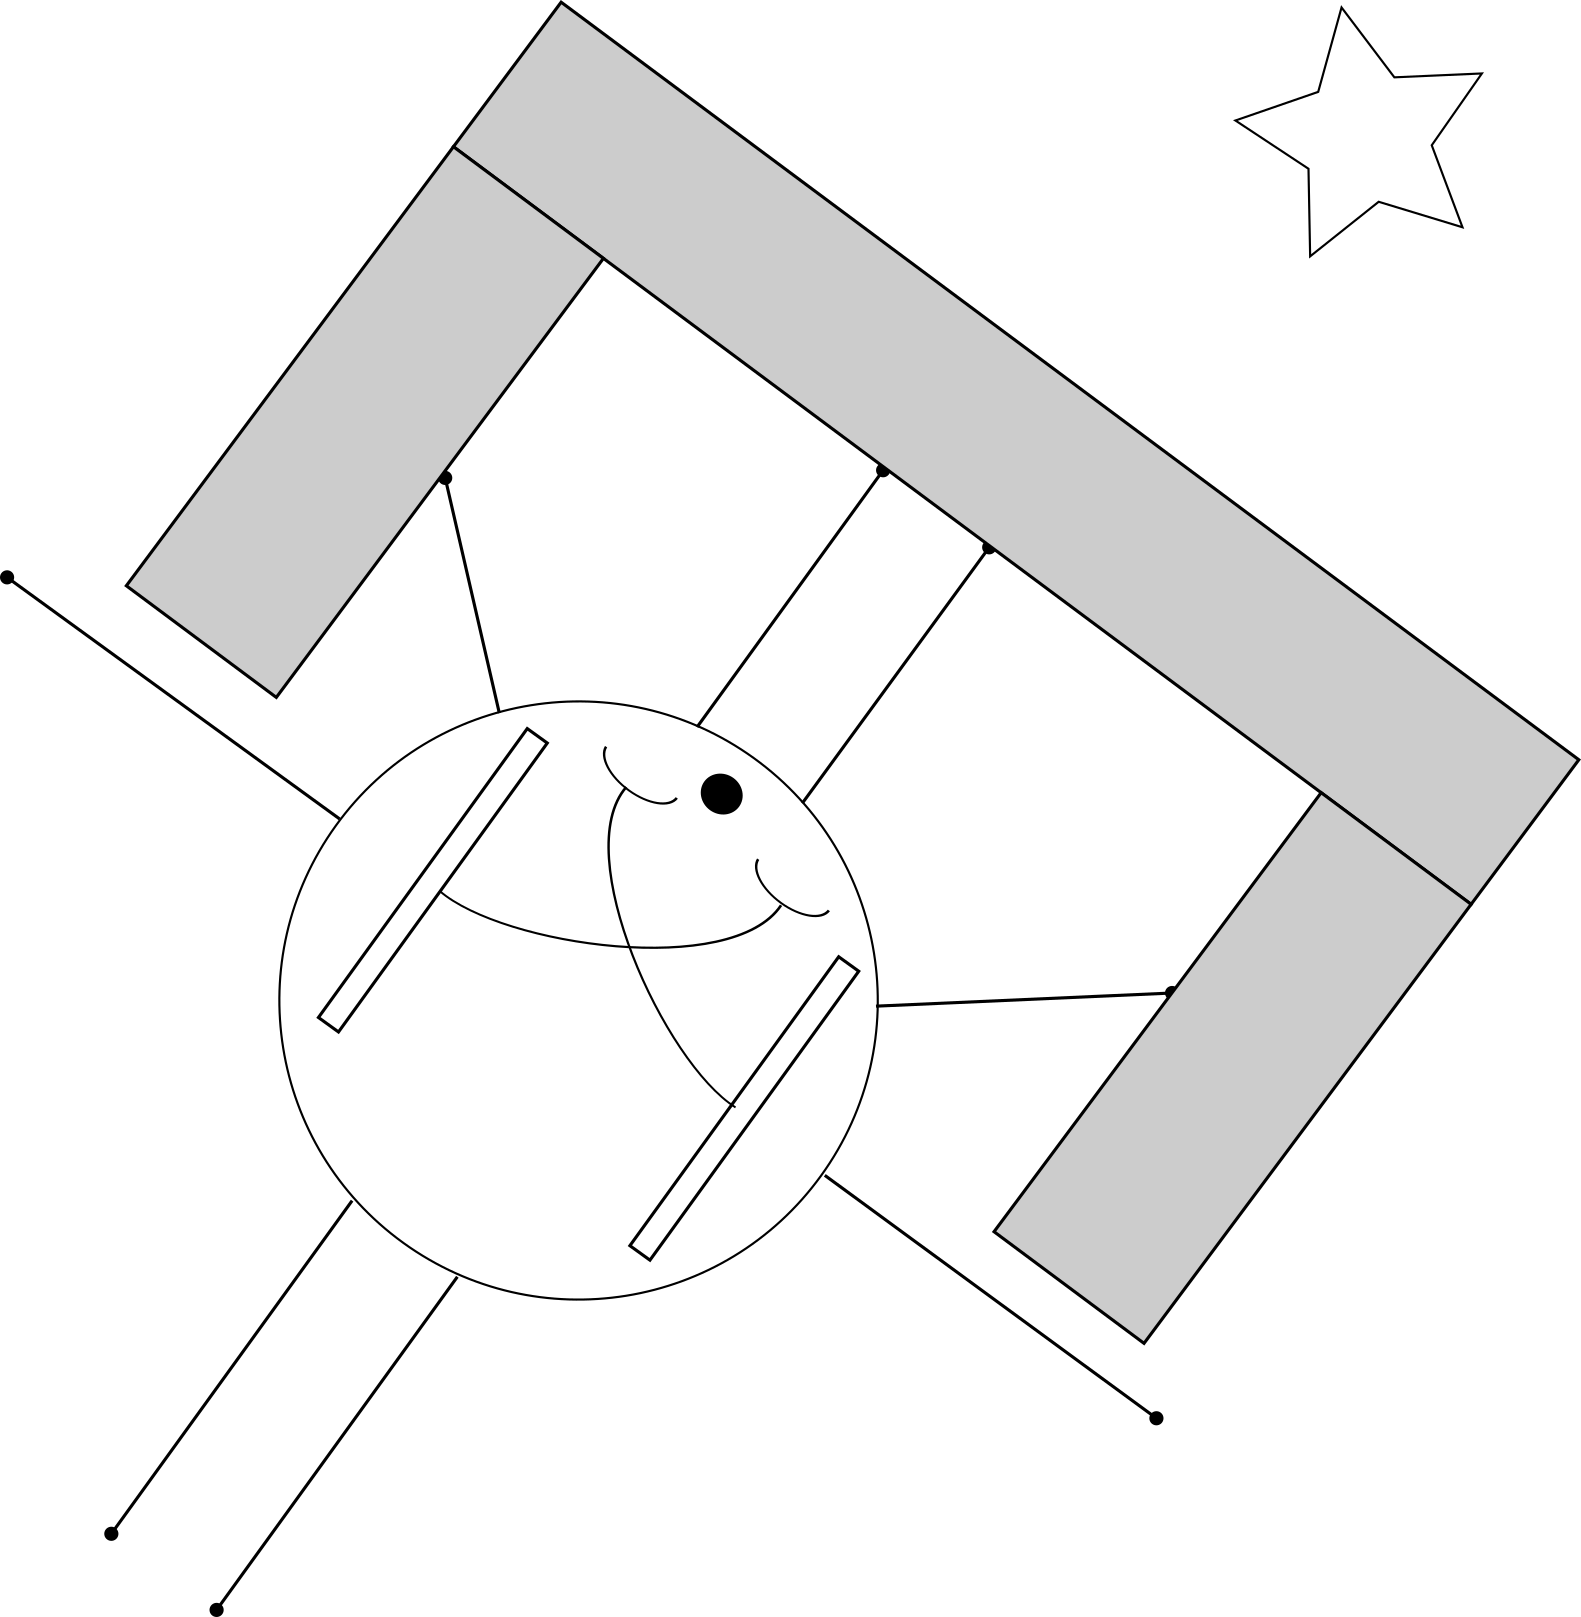
\includegraphics[width=0.8\columnwidth]{figs/uobstacle.png}
\caption{\label{fig:uobstacle}A differential wheel robot with distance and light sensors wired in a ``light following'' configuration in an U-shaped obstacle. Although the obstacle will be avoided, the light following behavior will continuously drive the robot into the obstacle unless state is added.}
\end{figure}


In order to avoid this situation, the robot needs to memorize its previous state and switch behaviors accordingly. For example, in addition to the basic combined avoidance and following behavior (``avoid and follow''), we can introduce an additional term (``wall following') in which the robot uses its proximity sensors to maintain a constant distance to a wall. In order to switch from one to the other behavior, we need to change the constant gains into dynamic ones that change their value based on other observations the robot makes. For example, the robot could estimate its progress by monitoring whether its light sensor is constantly increasing, and if it is not, inhibiting phototaxis behavior and emphasizing wall following. 

While feasible and potentially realizable with simple analog electronics, designing reactive systems with time-dependent behavior and state very quickly becomes difficult to manage. It is therefore desirable to establish discrete abstractions for various behaviors, which can be more easily managed and understood by a programmer. 
%
%
\section{Finite State Machines}\label{sec:fsm}
A simple, yet powerful tool to facilitate switching between different behaviors is a so-called \emph{Finite State Machine} (FSM)\index{Finite State Machine}\index{FSM}. In an FSM, each state is associated with a specific controller. In practice, an FSM consists of a global variable that stores the current state and a series of ``if'' statements that contain the code that is associated with each unique state. For example, an FSM to perform phototaxis while avoiding U-obstacles could consist of two states, with one for each desired behavior: one state that computes wheel-speeds so the robot moves toward the light while using its sensors to avoiding obstacles ahead of it, and another state that computes wheel-speeds so the performs a wall following behavior. To specify an FSM, one also needs to specify the \emph{state transitions}\index{state transition}\index{transition (state)}, the conditions that determine when to switch which state the FSM is in. For example, if multiple sensors detect an obstacle (implying that it may be a large one), then it may be desirable to have the FSM transition from its first state (phototaxis with simple obstacle avoidance) to its second (wall following). Finally, it is necessary to specify an initial state (the state the system starts in) and any final states (terminal states that signify program termination). An FSM can be depicted graphically, as shown in Figure \ref{fig:fsm_example}.

\todo{Insert FSM figure}
\begin{figure}
\caption{A simple Finite State Machine (FSM) with two states, an initial state, state transitions, and conditions that trigger a state transition.}
\end{figure}

Formally, a FSM is defined by a Tuple $(\Sigma, S, s_0, \delta, F)$ where:
\begin{itemize}
\item $\Sigma$ is the input \emph{Alphabet}, a set of symbols that represent events that can trigger state transitions,
\item $S$ is a finite set of states,
\item $s_0$ is an initial state, an element of $S$, that is $s_i \in S$,
\item $\delta$ is the state-transition function $\delta: S \times \Sigma \rightarrow S$ that maps combinations of states in $S$ and symbols $x$ in $\Sigma$ to a new state in $S$, and
\item $F$ is the set of final states, a subset of $S$. 
\end{itemize}

Historically, this definition stems from FSMs formally defining the working of a computer with a stream of symbolic commands of an actual program. In robotics, symbols that trigger state transitions can themselves be the result of complex computations. For example, a robot might switch to wall-following if it has not made actual progress toward its goal in some time and resume phototaxis once it reached a position that is closer to the light than it was before. 

In conjunction with a controller for each state, an FSM is called a \emph{Hybrid System}\cite{van2000introduction} as it combines both discrete (the state) and continuous (the controller outputs) variables. 

\subsection{Implementation}
A low-level robot controller is usually implemented as a loop with fixed loop time, for example 100ms for slow moving differential-wheel robots and 1ms for dynamical systems such as drones. At each start of the loop, the controller reads all sensors, then branches into the part of the code that corresponds to its current state, processes sensor information and computes actuator output, and finally sends the control commands to the actuators. 

Unlike a computer program that can process information as fast as possible, the robot controller needs to wait until sensor information are actually available, and actuator commands are executed (i.e. that the robot has physically moved). As the robot keeps moving while computation is ongoing, it is important to run the main loop at a constant rate. As computation is usually much faster than the loop time, it might be necessary to use an internal clock to wait until the loop time is expired. 


%@book{van2000introduction,
%  title={An introduction to hybrid dynamical systems},
%  author={Van Der Schaft, Arjan J and Schumacher, Johannes Maria},
%  volume={251},
%  year={2000},
%  publisher={Springer London}
%}



\begin{enumerate}
\item State is kept by a global variable
\item Robot program is executed in a loop, switch statement is used to enter different branches
\item Each state includes conditionals that set next state
\item Loop execution time is constant, usually done via sleep statements. This is important as odometry computations require a constant time to function.
\item FSMs are difficult to maintain. Adding a state requires modifiying the transitions of all states leading into that state and possibly also out of that new state.
\end{enumerate}

\section{Hierarchical Finite State Machines}\label{sec:stateflow}
\begin{enumerate}
\item FSMs are grouped into clusters, creating super-states
\item Also known as ``Statecharts'' \cite{harel1987statecharts}

\item State transitions between super states can be tied to states in the included FSM or be implicitly connected to all states of the included FSM, which allows leaving the super state from every state therein.
\item Super states can also be executed in parallel, providing events that lead to state transitions in other FSMs
\item Robot control software like ROS, LCM, or Yarp provide frameworks to implement asynchronous Hierarchical FSMs (HFSM), allowing super-states to subscribe to messages published by other super-states as well as directly triggering state transitions across different processes running in parallel in a service model.
\item HFSM solve some of the problems of FSMs by increasing modularity, simplifying programmability, but still have the problem that $N$ states can lead to $N^2$ state transitions, each of which need to be manually coded.
\end{enumerate}

\section{Behavior Trees}\label{sec:behaviortrees}
\begin{figure}
    \centering
    \begin{forest}
    {for tree={%
        minimum height = 4ex, 
        minimum width = 4ex, 
        draw, 
        parent anchor=south, 
        child anchor=north, 
        align=center
        }
    }
        [{\scriptsize Tilt Insert}\\ $\longrightarrow^*$
            [\scriptsize Rotate\\ $\theta_{tilt}$]
            [\scriptsize Move to\\ \scriptsize Contact \normalsize $-Z$]
            [\scriptsize Rotate\\ $-\theta_{tilt}-\delta \theta$]
            [\scriptsize Rotate\\ $\delta \theta$]
            [\scriptsize Hand at\\ $Z_{insert}$, ellipse]
        ]
    \end{forest}
    \caption{Tilt Insert Skill BT. The sequence first ..., then moves downwards until contact is made, rotates ... }
    \label{BTtilt}
\end{figure}

\begin{enumerate}
\item Programs are organized into nodes, each implementing certain functionality.
\item A node can have sub-nodes, like leafs of a tree, that are sequentially executed.
\item Each node can be \emph{running}, \emph{failed}, or \emph{successful}.
\item Execution within a node is triggered by a so-called \emph{tick} received by its parent node.
\item Nodes report their state back to their parent node.
\item A parent node issues ticks to its child nodes one by another, only moving to the next of its child nodes once the last one has returned \emph{successful}. (Or when a single one returns successful: ``Any" vs. ``All" type node)
\item As long as a child node is returning \emph{running}, it continues to receive ticks.
\item If a node fails, this information can be processed by the parent node who either passes it up, or restart the sequence of child nodes.
\item Popular in video game AI, give Minecraft example
\end{enumerate}

\section{Mission Planning}\label{sec:strips}
\begin{enumerate}
\item The original GPS algorithm: operations that transform a set of pre-conditions into a set of post-states, and search thereon
\item Mission planning with BTs
\end{enumerate}

\section{Exercises}

\begin{enumerate}
\item A differential wheel robot has three downward-facing light sensors at its tip. The sensors are spaced such that the robot can detect a black line on a white ground. Derive the equations for a line-following robot using the Braitenberg formalism.
\item Derive a control scheme that combines line following and obstacle avoidance. Discuss your choices assuming that the robot has to avoid obstacles at all cost. 
\item Use a robotic simulator of your choice to implement basic phototaxis and obstacle avoidance. 
\item Use a robotic simulator of your choice to implement basic wall-following behavior
\item Implement a simple finite state machine that combines obstacle avoidance, phototaxis and wall-following and is capable to escape from a U-shaped obstacle
\item A FSM implements the following behavior: perform photo-taxis until an obstacle is it; then perform wall-following for 10 time steps. Draw an appropriate Finite State Machine. How many states do you need?
\item A robot runs at a 100ms loop time. Performing sensor readings takes 3ms, odometry computations 15ms, and executing logic takes 30ms on average. Which of these operations is likely to fail if the task logic takes 80ms?
\item Formulate both a Finite State Machine and a Behavior tree for the game ``Rats Life'', label each state and conditional transition, and compare the two representations.
\end{enumerate}
